\documentclass[11pt,a4paper]{article}
\usepackage[margin=2.2cm]{geometry}
\usepackage{amsmath,amssymb,booktabs,graphicx,xcolor,enumitem,array,tabularx,hyperref,float,caption}
\usepackage[most]{tcolorbox}
\usepackage{tikz}
\usetikzlibrary{arrows.meta,positioning,shapes.geometric}
\usepackage{listings}
\hypersetup{colorlinks=true,linkcolor=blue!50!black,urlcolor=blue!50!black,citecolor=blue!50!black}
\captionsetup{font=small,labelfont=bf}
\setlist{itemsep=0.25em,topsep=0.3em}

% ---------------------------------------------------------------- colour code for quantities
\definecolor{ecol}{RGB}{192,57,43}     % energies
\definecolor{mucol}{RGB}{142,68,173}   % chemical potentials
\definecolor{gcol}{RGB}{22,50,92}      % geometry
\definecolor{tcol}{RGB}{230,126,34}    % terminations
\newcommand{\Ef}{\textcolor{ecol}{E_{\mathrm{form}}}}
\newcommand{\Eh}{\textcolor{ecol}{E_{\mathrm{hull}}}}
\newcommand{\Etot}{\textcolor{ecol}{E}}
\newcommand{\dmu}{\textcolor{mucol}{\Delta\mu_{\mathrm F}}}
\newcommand{\dmustar}{\textcolor{mucol}{\Delta\mu_{\mathrm F}^{*}}}
\newcommand{\muzero}{\textcolor{mucol}{\mu^{0}}}
\newcommand{\dG}{\textcolor{ecol}{\Delta G}}
\newcommand{\alat}{\textcolor{gcol}{a}}
\newcommand{\Area}{\textcolor{gcol}{A}}
\newcommand{\Tm}{\textcolor{tcol}{T}}
\newcommand{\gam}{\textcolor{ecol}{\gamma}}
\lstset{basicstyle=\ttfamily\small,columns=fullflexible,frame=single,backgroundcolor=\color{gray!6},rulecolor=\color{gray!40},
        breaklines=true,xleftmargin=0.5em,xrightmargin=0.5em}
\newtcolorbox{learn}[1][]{colback=blue!3,colframe=blue!45!black,fonttitle=\bfseries,title=#1,boxrule=0.6pt,arc=2pt}
\newtcolorbox{caveat}[1][]{colback=red!3,colframe=red!55!black,fonttitle=\bfseries,title=#1,boxrule=0.6pt,arc=2pt}

\title{\textbf{Thermodynamic stability of the MXenes Cr$_2$CF$_2$, Ni$_2$NF$_2$ and Mo$_2$C}\\[0.3em]
\large Convex hulls, phase diagrams and termination chemistry with \texttt{symphase mxene} --- a worked report you can reuse for other 2D materials}
\author{Gokaran Shukla\\ \small KAUST}
\date{\small November 2026 \;·\; SymPhase module \texttt{symphase.twod}}

\begin{document}
\maketitle

\begin{tcolorbox}[colback=gray!4,colframe=gray!50,title=\textbf{Summary},fonttitle=\bfseries]
\begin{itemize}
\item Three monolayer MXenes were built, relaxed and placed in the convex hull of all relevant bulk phases:
F-terminated Cr$_2$CF$_2$ and Ni$_2$NF$_2$, and bare Mo$_2$C.
\item All three are \textbf{metastable}: $\Eh = 265$, $377$ and $391$ meV/atom. This is the expected range for MXenes, which are made
top-down by etching and not by equilibrium synthesis.
\item Lowest-energy decompositions: \;7\,Cr$_2$CF$_2\to$ Cr$_7$C$_3$ + 4\,C + 7\,CrF$_2$ \;·\; 3\,Ni$_2$NF$_2\to$ Ni$_3$N + N$_2$ + 3\,NiF$_2$ \;·\;
Mo$_2$C(2D) $\to$ bulk $\beta$-Mo$_2$C (surface energy $\gam = 1.23$ J/m$^2$).
\item Fluorine prefers the \textbf{fcc} hollow site (the hcp site costs $\approx$\,0.1 eV/atom). F termination beats the bare sheet for
$\dmu > \dmustar = -3.90$ (Cr$_2$C), $-2.92$ (Ni$_2$N) and $-2.95$ eV (Mo$_2$C), so under practically any fluorinating condition.
\item Energies come from the universal machine-learned potential CHGNet, on the Materials Project PBE/PBE+U scale. Bulk formation energies
agree with experiment to $\lesssim$\,0.07 eV/atom for the fluorides and carbides that control the hulls. These are \textbf{screening}
results: Section~\ref{sec:apply} explains how to confirm them with VASP.
\end{itemize}
\end{tcolorbox}

\tableofcontents
\newpage

% =============================================================================
\section{What is being calculated, and why}
\label{sec:concepts}

\subsection{MXenes in one paragraph}
MXenes are two-dimensional transition-metal carbides and nitrides with formula $M_{n+1}X_n\Tm_x$. Here $M$ is an early or middle transition metal,
$X$ = C or N, and \Tm\ is a surface termination (F, O, OH, Cl, \dots) picked up during synthesis. They are obtained by selectively etching
the A layer out of a layered MAX phase (e.g.\ Ti$_3$AlC$_2$ in HF), followed by delamination. Structurally, $n+1$ close-packed metal layers
sandwich $n$ layers of $X$ in octahedral sites, stacked $ABC$ as in the parent MAX phase. The terminations sit in hollow sites above the outer
metal layers.

\begin{learn}[Point 1 --- the formula tells you the structure]
$M_2X\Tm_2$ ($n=1$): metal / $X$ / metal plus one termination on each side, so 5 atoms per primitive cell.\;
$M_3X_2\Tm_2$ ($n=2$): 7 atoms.\; Double-metal ordered MXenes such as Mo$_2$TiC$_2$O$_2$ put one metal on the outer layers and the other inside.
\texttt{symphase mxene} builds all of these from the answers to its questions (metal, $X$, $n$, passivation, site).
\end{learn}

\subsection{Formation energy, convex hull and energy above the hull}
For a compound with total energy $\Etot$ and $N_i$ atoms of element $i$,
\begin{equation}
\Ef = \frac{\Etot - \sum_i N_i\,\muzero_i}{\sum_i N_i}\qquad[\text{eV/atom}],
\end{equation}
where $\muzero_i$ is the energy per atom of element $i$ in its reference state: bcc Cr/Mo, fcc Ni, graphite, and the molecular crystals
of N$_2$ and F$_2$. Plotting $\Ef$ of every known phase against composition and taking the lower convex envelope gives the \emph{convex hull}.
Phases on the hull are thermodynamically stable at $T=0$. Every other phase has a positive \emph{energy above the hull}
\begin{equation}
\Eh = \Ef - E_{\mathrm{form}}^{\mathrm{hull}}(\text{same composition}) \ge 0 ,
\end{equation}
which is the energy (per atom) released if it decomposes into the hull phases at its composition: its \emph{decomposition products}.

\begin{learn}[Point 2 --- how to read the three numbers]
\begin{itemize}
\item $\Ef < 0$: more stable than the elements. This alone does \emph{not} mean stable; it only beats the trivial competitors.
\item $\Eh$: the only stability measure that accounts for \emph{all} competing phases. It is never negative for a
phase that is already in the hull data.
\item The decomposition products tell you \emph{which} phases the material would turn into. That points to the competing
phases whose energies must be accurate.
\end{itemize}
\end{learn}

\subsection{Why 2D materials are always above the bulk hull}
A free-standing sheet has two surfaces per primitive cell. Its energy per atom therefore lies above that of bulk phases of the same
composition by roughly twice the surface energy divided by the number of atoms. Typical MXenes sit a few hundred meV/atom above the hull,
yet they are routinely synthesised. The relevant questions are \emph{relative}: which termination, which metal, which $n$ gives the lowest
$\Eh$, and whether the decomposition products are kinetically accessible.

\begin{learn}[Point 3 --- interpreting $\Eh$ for 2D materials]
Do not apply the bulk rule of thumb ($\Eh\lesssim 50$ meV/atom $\Rightarrow$ synthesizable) to monolayers. Compare MXenes
\emph{with each other} with the same method, and compare with known MXenes (e.g.\ Ti$_3$C$_2$T$_x$, Mo$_2$CT$_x$) as benchmarks. For a bare sheet with a bulk polymorph of the
same composition, $\Eh$ is literally the surface cost: $\gam = \Eh N/(2\Area)$.
\end{learn}

\subsection{Termination chemistry: a phase diagram in chemical potential}
Whether a sheet is terminated depends on the chemical environment, i.e.\ the fluorine chemical potential $\mu_{\mathrm F} = \muzero_{\mathrm F} + \dmu$
($\dmu = 0$ is the F$_2$ reference; lower values mean less fluorinating conditions). Per primitive cell of area \Area,
\begin{equation}
\dG(\dmu) = \frac{\Etot(M_2XF_2) - \Etot(M_2X) - 2\muzero_{\mathrm F} - 2\dmu}{\Area}.
\end{equation}
The F-terminated sheet is favoured where $\dG<0$, i.e.\ for $\dmu > \dmustar = [\Etot(M_2XF_2) - \Etot(M_2X) - 2\muzero_{\mathrm F}]/2$.
$\dmustar$ is the binding energy per F atom relative to F$_2$.

% =============================================================================
\section{Method --- the workflow step by step}
\label{sec:method}

\begin{figure}[H]
\centering
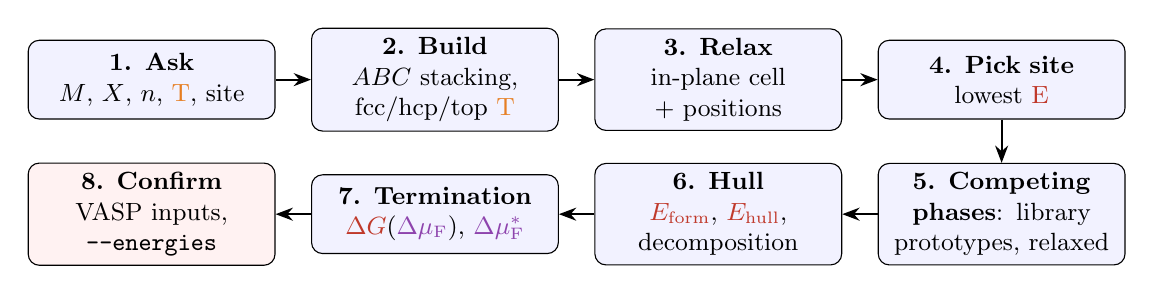
\begin{tikzpicture}[node distance=0.55cm and 0.45cm, every node/.style={font=\small},
  box/.style={draw, rounded corners, fill=blue!5, align=center, minimum height=1.0cm, text width=2.9cm},
  arr/.style={-{Stealth[length=2.2mm]}, thick}]
\node[box] (q) {\textbf{1. Ask}\\ $M$, $X$, $n$, \Tm, site};
\node[box, right=of q] (b) {\textbf{2. Build}\\ $ABC$ stacking,\\ fcc/hcp/top \Tm};
\node[box, right=of b] (r) {\textbf{3. Relax}\\ in-plane cell\\ + positions};
\node[box, right=of r] (s) {\textbf{4. Pick site}\\ lowest \Etot};
\node[box, below=of s] (l) {\textbf{5. Competing}\\ \textbf{phases}: library\\ prototypes, relaxed};
\node[box, left=of l] (h) {\textbf{6. Hull}\\ $\Ef$, $\Eh$,\\ decomposition};
\node[box, left=of h] (t) {\textbf{7. Termination}\\ $\dG(\dmu)$,\ $\dmustar$};
\node[box, left=of t, fill=red!5] (v) {\textbf{8. Confirm}\\ VASP inputs,\\ \texttt{--energies}};
\draw[arr] (q) -- (b); \draw[arr] (b) -- (r); \draw[arr] (r) -- (s); \draw[arr] (s) -- (l);
\draw[arr] (l) -- (h); \draw[arr] (h) -- (t); \draw[arr] (t) -- (v);
\end{tikzpicture}
\caption{Workflow of \texttt{symphase mxene --hull}. Steps 1--7 run automatically; step 8 is the DFT follow-up.}
\end{figure}

\paragraph{Step 1 --- input (interactive).} Without arguments the program asks:
\begin{lstlisting}
$ symphase mxene --hull
  transition metal M (e.g. Cr, Mo, Ti; ordered double-M as outer,inner e.g. Mo,Ti): Cr
  X element (C or N) [C]: C
  n in M(n+1)X(n) (1, 2, 3) [1]: 1
  passivation / termination (F, O, OH, Cl, Br, S, none) [F]: F
  termination site (fcc, hcp, top, auto = lowest energy) [auto]: auto
\end{lstlisting}
The same run without questions: \texttt{symphase mxene --M Cr --X C --T F --hull --vasp}.

\paragraph{Step 2 --- structure.} The $2n+1$ metal/$X$ layers are placed on the $B,A,C,B,\dots$ sites of a hexagonal lattice, with a
starting lattice constant $\alat_0 = 2.36\,r_M$ ($r_M$ = metallic radius). The interlayer spacing is 1.15~Å and the vacuum 20~Å.
Terminations go on both surfaces:
\textbf{fcc} = the hollow above the metal of the \emph{opposite} side (``model I''); \textbf{hcp} = above $X$ (``model II'');
\textbf{top} = above the outer metal. OH is built as O plus H 0.97~Å above it.

\paragraph{Step 3 --- relaxation.} All atomic positions and the \emph{in-plane} lattice are relaxed (FIRE + Fréchet cell filter with
the $c$ axis masked, so the vacuum is kept) until forces fall below 0.02 eV/Å. A 0.02~Å random displacement breaks the
starting symmetry, so that distortions can develop.

\paragraph{Step 4 --- termination site.} Each site is relaxed and the lowest energy is kept (\texttt{site=auto}). Two sites
are counted as the same when their energies differ by less than 1 meV/atom (a ``top'' start often slides into the fcc hollow).

\paragraph{Step 5 --- competing phases.} SymPhase contains a library of crystallographic prototypes (space group, lattice and Wyckoff
parameters from the AFLOW prototype encyclopedia and ICSD refinements; Table~\ref{tab:library}). It takes every phase whose elements are a
subset of the MXene's, relaxes it fully with the same energy model, and caches the result (\texttt{library\_chgnet.json}). You can add
your own phases with \texttt{--extra POSCAR/CIF}.

\paragraph{Step 6 --- hull.} The MXene and the library phases form the convex hull (pymatgen phase diagram, via
\texttt{symphase.hull.HullAnalysis}). The output gives $\Ef$, $\Eh$, the decomposition, \texttt{hull.json} and \texttt{phase\_diagram.png}.

\paragraph{Step 7 --- termination diagram.} The bare sheet is relaxed too, and $\dG(\dmu)$ and $\dmustar$ follow from Eq.~(3) with
$\muzero_{\mathrm F}$ = the energy per atom of the relaxed F$_2$ molecular crystal (function \texttt{termination\_\allowbreak energies}).

\paragraph{Energy model.} No database download is needed. Energies are computed with \textbf{CHGNet}~\cite{chgnet}, a graph-neural-network
interatomic potential trained on the Materials Project relaxation trajectories~\cite{mp}. Its energies are on the MP2020-compatible PBE/PBE+U
scale, so metals, carbides, nitrides and fluorides can be combined in one hull. CHGNet also predicts magnetic moments but does not
constrain a magnetic order.

% =============================================================================
\section{How good is the energy model? Validation on the bulk phases}
\label{sec:validation}

\begin{table}[H]
\centering\small
\caption{Formation energies (eV/atom) of the competing bulk phases: CHGNet (this work) versus approximate experimental formation
enthalpies at 298~K from standard thermochemical tables. Check the experimental values against the original sources before citing.}
\label{tab:validation}
\begin{tabular}{@{}lllrrr@{}}
\toprule
phase & prototype & space group & $\Ef$ CHGNet & $\Delta H_f$ exp. & difference\\
\midrule
CrF$_2$ & rutile (distorted) & $P4_2/mnm$ start & $-2.754$ & $-2.69$ & $-0.07$\\
CrF$_3$ & VF$_3$ / D0$_{12}$ & $R\bar3c$ & $-2.933$ & $-3.00$ & $+0.07$\\
NiF$_2$ & rutile & $P4_2/mnm$ & $-2.207$ & $-2.25$ & $+0.04$\\
Cr$_3$C$_2$ & tongbaite D5$_{10}$ & $Pnma$ & $-0.163$ & $-0.18$ & $+0.01$\\
Cr$_7$C$_3$ & D10$_1$ & $Pnma$ & $-0.201$ & $-0.17$ & $-0.03$\\
Cr$_{23}$C$_6$ & D8$_4$ & $Fm\bar3m$ & $-0.166$ & $-0.15$ & $-0.02$\\
$\beta$-Mo$_2$C & & $Pbcn$ & $-0.179$ & $-0.16$ & $-0.02$\\
Ni$_3$N & $\varepsilon$-Fe$_3$N & $P6_322$ & $-0.048$ & $+0.00$ & $-0.05$\\
MoC & WC & $P\bar6m2$ & $+0.007$ & $-0.15$ & $+0.15$\\
\bottomrule
\end{tabular}
\end{table}

\begin{learn}[Point 4 --- what the validation tells you]
\begin{itemize}
\item The phases that \emph{control} the three hulls (CrF$_2$, Cr$_7$C$_3$, NiF$_2$, Ni$_3$N, $\beta$-Mo$_2$C) are reproduced to within 0.07 eV/atom.
\item Cr$_3$C$_2$ lies 9 meV/atom above the CHGNet hull, although it is stable experimentally. This is within the model error and does not
affect the MXene results.
\item MoC is underbound by 0.15 eV/atom, a known kind of failure for refractory carbides. It does not enter the Mo$_2$C decomposition,
but it would matter for C-rich Mo compounds.
\item NiF$_3$ appears on the hull, whereas experimentally it is not stable. Again it plays no role here.
\item Always check the decomposition products: only their energies (and the MXene's) enter $\Eh$.
\end{itemize}
\end{learn}

% =============================================================================
\section{Results}
\label{sec:results}

\begin{figure}[H]
\centering
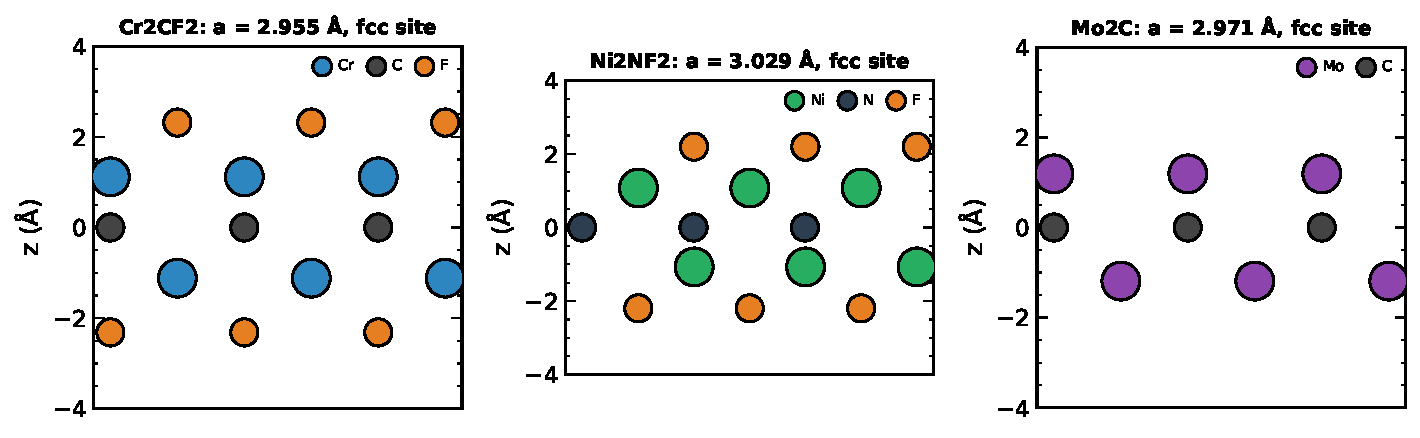
\includegraphics[width=\textwidth]{figures/mxene_structures.pdf}
\caption{Relaxed monolayers, side view along $[1\bar10]$ (three cells). Large circles: metal; dark: C/N; orange: F.}
\label{fig:structures}
\end{figure}

\begin{table}[H]
\centering\small
\caption{Relaxed geometry and energetics. $\Delta E_{\mathrm{site}}$ = $E(\text{hcp}) - E(\text{fcc})$; $\Delta E_{\mathrm{dec}}$ = decomposition
energy per formula unit ($\Eh\times N$) and per area; $m_M$ = CHGNet local moment on the metal (indicative only).}
\label{tab:results}
\begin{tabular}{@{}lccc@{}}
\toprule
 & Cr$_2$CF$_2$ & Ni$_2$NF$_2$ & Mo$_2$C (bare)\\
\midrule
lattice constant \alat\ (Å) & 2.955 & 3.029 & 2.971\\
sheet thickness (outer atoms, Å) & 4.63 & 4.40 & 2.38\\
$M$--$X$ / $M$--F / $M$--$M$ bonds (Å) & 2.04 / 2.08 / 2.81 & 2.03 / 2.07 / 2.77 & 2.09 / -- / 2.93\\
termination site & fcc & fcc & --\\
$\Delta E_{\mathrm{site}}$ (meV/atom) & +105 & +101 & --\\
$\Ef$ (eV/atom) & $-1.445$ & $-0.959$ & $+0.212$\\
$\Eh$ (meV/atom) & 265 & 377 & 391\\
$\Delta E_{\mathrm{dec}}$ (eV/f.u.) \;/\; (eV/Å$^2$) & 1.32 / 0.175 & 1.89 / 0.238 & 1.17 / 0.153\\
decomposition & Cr$_7$C$_3$ + C + CrF$_2$ & Ni$_3$N + N$_2$ + NiF$_2$ & $\beta$-Mo$_2$C\\
$\dmustar$ for F termination (eV) & $-3.90$ & $-2.92$ & $-2.95$ (hcp)\\
$m_M$ ($\mu_B$) & 2.4 & 0.8 & 0.0\\
\bottomrule
\end{tabular}
\end{table}

% -----------------------------------------------------------------------------
\subsection{Cr$_2$CF$_2$}

\begin{figure}[H]
\centering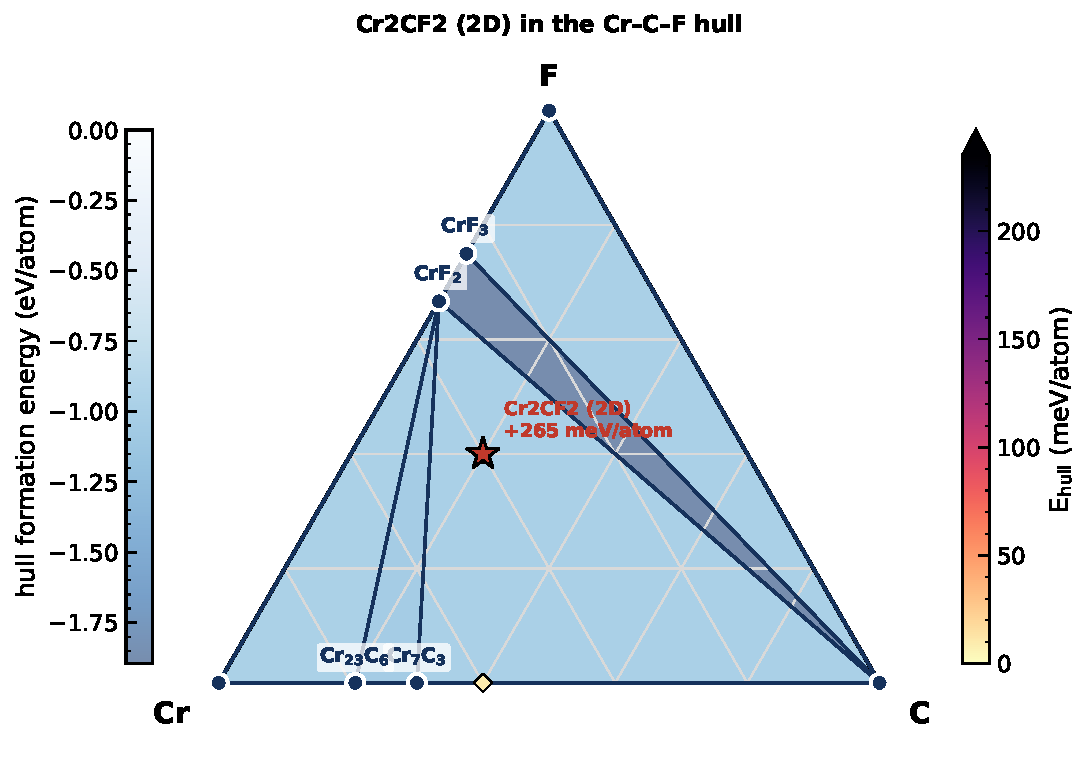
\includegraphics[width=0.62\textwidth]{figures/mxene_pd_Cr2CF2.pdf}
\caption{Cr--C--F phase diagram (Gibbs triangle). Dots: stable phases. Lines: hull tie-lines. Star: the Cr$_2$CF$_2$ monolayer. Its composition
lies inside the Cr$_7$C$_3$--C--CrF$_2$ triangle, which therefore gives the decomposition products.}
\label{fig:cr}
\end{figure}

\begin{enumerate}[label=\textbf{Cr.\arabic*}]
\item \textbf{Termination site.} F relaxes into the fcc hollow. Starting on top of Cr ends in the same state (energies equal to $10^{-4}$ eV/atom).
The hcp site (above C) is 105 meV/atom higher, and the sheet contracts there to $\alat = 2.76$~Å: F above C pulls the outer Cr inwards.
\item \textbf{Geometry.} $\alat = 2.955$~Å. Fluorination expands the bare Cr$_2$C sheet ($\alat = 2.78$~Å) by 6\%, because F withdraws electrons
from the Cr--Cr bonds. The Cr--C distance of 2.04~Å is close to that in Cr carbides (2.0--2.1~Å).
\item \textbf{Formation energy.} $\Ef = -1.445$ eV/atom is strongly negative, almost entirely because of the Cr--F bonds (CrF$_2$ has $\Ef = -2.75$ eV/atom).
\item \textbf{Hull.} The stable phases are Cr, C, F$_2$, Cr$_{23}$C$_6$, Cr$_7$C$_3$, CrF$_2$ and CrF$_3$. Cr$_2$CF$_2$ lies 265 meV/atom above the hull.
\item \textbf{Decomposition.} Per atom: 0.29 Cr$_7$C$_3$ + 0.11 C + 0.60 CrF$_2$ (atom fractions). As a balanced reaction:
\[7\,\mathrm{Cr_2CF_2}\;\to\;\mathrm{Cr_7C_3} + 4\,\mathrm{C} + 7\,\mathrm{CrF_2},\qquad \Delta E = -1.32\ \text{eV per Cr}_2\text{CF}_2.\]
Chemically, the F-bound Cr becomes Cr(II) fluoride, and the remaining Cr cannot hold all the carbon, so graphite is released.
\item \textbf{Lesson.} Of the three, Cr$_2$CF$_2$ has the \emph{lowest} $\Eh$, because Cr--F bonding is strong. Fluorination stabilises
the sheet strongly ($\dmustar = -3.90$ eV, the most negative of the three).
\item \textbf{Magnetism.} CHGNet predicts about 2.4\,$\mu_B$ per Cr, so Cr$_2$CF$_2$ is magnetic. In DFT, compare ferromagnetic and
antiferromagnetic orders (the ground state of Cr-based MXenes is often AFM) and use PBE+U for Cr. This can shift $\Eh$ by tens of meV/atom.
\end{enumerate}

% -----------------------------------------------------------------------------
\subsection{Ni$_2$NF$_2$}

\begin{figure}[H]
\centering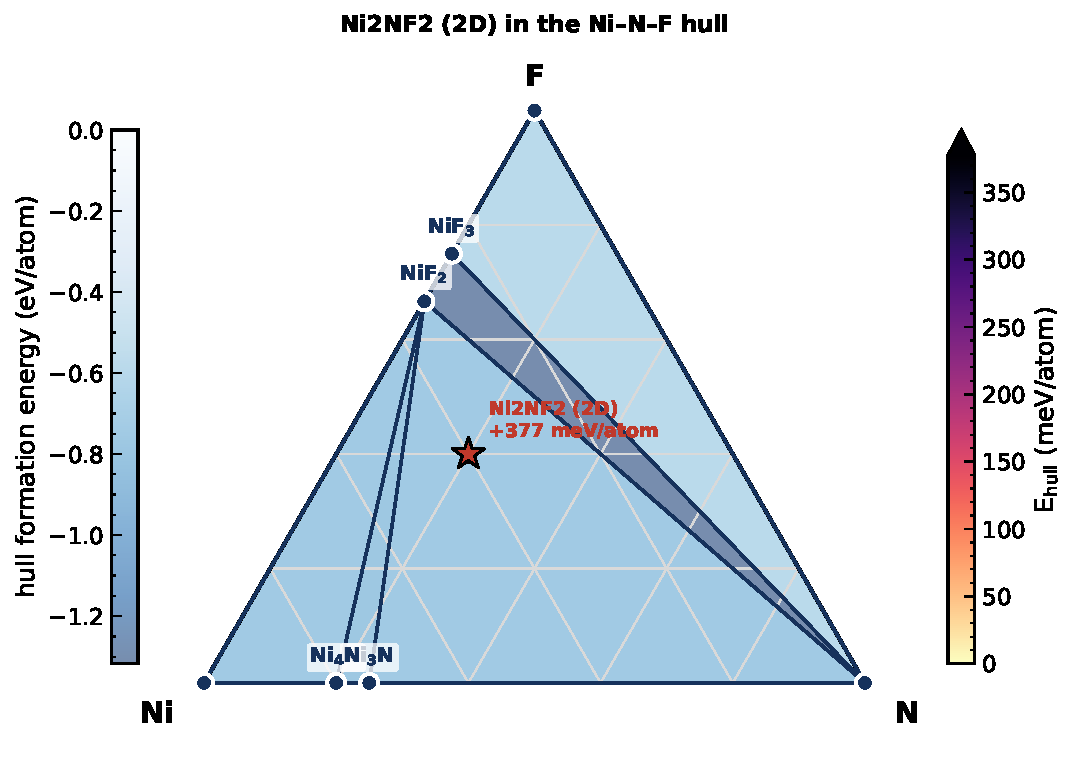
\includegraphics[width=0.62\textwidth]{figures/mxene_pd_Ni2NF2.pdf}
\caption{Ni--N--F phase diagram with the Ni$_2$NF$_2$ monolayer (star) inside the Ni$_3$N--N$_2$--NiF$_2$ triangle.}
\label{fig:ni}
\end{figure}

\begin{enumerate}[label=\textbf{Ni.\arabic*}]
\item \textbf{Termination site.} fcc again; hcp costs 101 meV/atom.
\item \textbf{Geometry.} $\alat = 3.029$~Å, a 13\% expansion relative to bare Ni$_2$N ($\alat = 2.67$~Å). This is the largest
fluorination-induced strain of the three, which signals strong Ni--F charge transfer.
\item \textbf{Formation energy.} $\Ef = -0.959$ eV/atom, less negative than for Cr$_2$CF$_2$. Ni--F bonds are weaker than Cr--F bonds
(NiF$_2$: $-2.21$ vs CrF$_2$: $-2.75$ eV/atom), and nickel nitrides are only marginally stable.
\item \textbf{Hull and decomposition.} $\Eh = 377$ meV/atom.
\[3\,\mathrm{Ni_2NF_2}\;\to\;\mathrm{Ni_3N} + \mathrm{N_2} + 3\,\mathrm{NiF_2},\qquad \Delta E = -1.89\ \text{eV per Ni}_2\text{NF}_2.\]
Half of the nitrogen is released as N$_2$. This is the hallmark of late-transition-metal nitrides, which are close to (or above) the
metal + N$_2$ line.
\item \textbf{Sensitivity (tested).} Ni$_3$N is overbound by about 0.05 eV/atom in CHGNet. Raising the Ni$_3$N and Ni$_4$N energies by
0.05 eV/atom (closer to experiment) removes them from the hull. The decomposition becomes 0.2 Ni + 0.2 N$_2$ + 0.6 NiF$_2$ (atom fractions),
and $\Eh$ \emph{decreases} from 377 to 365 meV/atom: a less stable competitor makes the MXene look \emph{less} unstable. The
conclusion is robust, and this is how to test the sensitivity of any result: shift the energy of each decomposition product
by its expected error and recompute.
\item \textbf{Lesson.} Nitride MXenes of late transition metals are the least stable class. Their stability depends on the nitrogen chemical
potential as well, so in a DFT study plot $\Eh$ (or the full grand-potential phase diagram) versus $\Delta\mu_{\mathrm N}$.
\end{enumerate}

% -----------------------------------------------------------------------------
\subsection{Mo$_2$C (bare)}

\begin{figure}[H]
\centering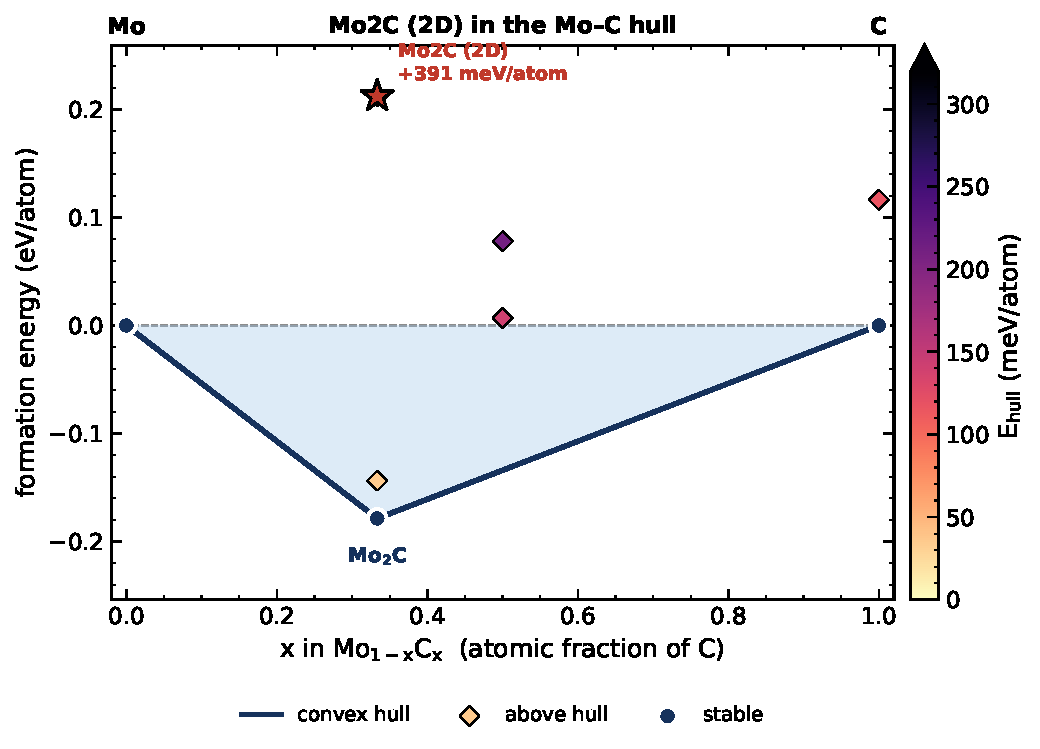
\includegraphics[width=0.58\textwidth]{figures/mxene_pd_Mo2C.pdf}
\caption{Mo--C binary hull. Bulk $\beta$-Mo$_2$C is the only stable compound. The bare Mo$_2$C monolayer (star) sits 391 meV/atom above it.
The diamonds are metastable polymorphs: hexagonal Mo$_2$C (+35), WC-type and NaCl-type MoC, and diamond.}
\label{fig:mo}
\end{figure}

\begin{enumerate}[label=\textbf{Mo.\arabic*}]
\item \textbf{Geometry.} $\alat = 2.971$~Å with a 2.38~Å thick Mo--C--Mo sandwich. Bulk $\beta$-Mo$_2$C has the same local Mo$_6$C octahedra;
the monolayer is essentially one slab cut from it.
\item \textbf{Formation energy.} $\Ef = +0.212$ eV/atom: the bare sheet is even less stable than Mo + graphite. The positive value
comes entirely from the two unsaturated Mo surfaces.
\item \textbf{Hull.} The decomposition is a single phase, 2D Mo$_2$C $\to$ bulk $\beta$-Mo$_2$C, so $\Eh$ is a pure surface energy:
\[\gam = \frac{\Eh\,N}{2\Area} = \frac{0.391\times 3}{2\times7.65}\ \text{eV/Å}^2 = 0.077\ \text{eV/Å}^2 = 1.23\ \text{J/m}^2 .\]
This is a typical value for a metallic carbide surface, and a good sanity check of the method.
\item \textbf{Termination.} Mo$_2$C binds F strongly ($\dmustar = -2.95$ eV), and here the \emph{hcp} site wins. The site preference depends on the metal,
which is why \texttt{site=auto} tests every site.
\item \textbf{Lesson.} Never judge a bare MXene by $\Ef$ alone. Compare it with bulk polymorphs of the same composition, and remember that real Mo$_2$C
sheets are terminated (O, OH, F), which removes most of this surface energy.
\end{enumerate}

% -----------------------------------------------------------------------------
\subsection{Termination phase diagram}
\begin{figure}[H]
\centering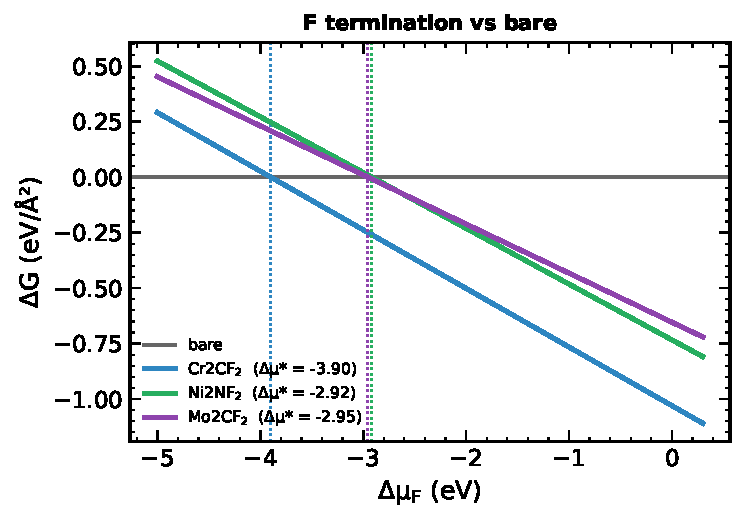
\includegraphics[width=0.6\textwidth]{figures/mxene_termination.pdf}
\caption{$\dG(\dmu)$ of F-terminated relative to bare sheets. Dotted lines mark $\dmustar$. To the right (more fluorinating), the F$_2$-terminated
sheet is stable.}
\label{fig:term}
\end{figure}

\begin{enumerate}[label=\textbf{T.\arabic*}]
\item $\dmustar$ is the energy gained per F atom on binding to the bare sheet, relative to F$_2$: $-3.90$ (Cr), $-2.92$ (Ni), $-2.95$ eV (Mo).
\item All three thresholds lie far below the F$_2$ reference ($\dmu=0$), so the terminated sheets are favoured unless the environment is
extremely F-poor. Fluorine terminations are therefore expected after fluoride-based etching.
\item The slope $-2/\Area$ is the same for all F$_2$-terminated sheets; only the intercept, i.e.\ the binding strength, differs. Several terminations
(F, O, OH) compete in the same way, each with its own chemical potential. With O and OH added this becomes a 2D (or 3D) Pourbaix-type diagram.
\end{enumerate}

% =============================================================================
\section{How to apply this to other materials}
\label{sec:apply}

\subsection{Recipe}
\begin{enumerate}[label=\textbf{Step \arabic*.},leftmargin=4.2em]
\item \textbf{Choose the chemistry.} Run \texttt{symphase mxene} and answer the questions, or pass e.g.\ \texttt{--M Ti --X C --n 2 --T O} for Ti$_3$C$_2$O$_2$,
\texttt{--M V --X C --T OH}, or \texttt{--M Mo,Ti --X C --n 2 --T O} for ordered Mo$_2$TiC$_2$O$_2$.
\item \textbf{Keep \texttt{--site auto}.} The preferred site changes with the metal (fcc for Cr and Ni, hcp for Mo with F).
\item \textbf{Inspect the competing phases.} Read the ``relaxing \dots'' lines. Is every known bulk phase of your system there? If not, add it:
\texttt{--extra Ti3AlC2.cif TiOF2.vasp}. Missing phases make $\Eh$ too \emph{small}, i.e.\ too optimistic.
\item \textbf{Read \texttt{hull.json}.} Note $\Ef$, $\Eh$ and the decomposition. Write the balanced reaction (Section~\ref{sec:results}) and ask whether the products are
chemically sensible.
\item \textbf{Validate the decomposition products.} Compare their $\Ef$ with experiment or the Materials Project (Table~\ref{tab:validation}); errors there translate
one-to-one into $\Eh$.
\item \textbf{Termination diagram.} Use \texttt{termination\_energies(M, X, n, ("F","O","OH"))} for $\dmustar$ of each termination.
\item \textbf{Confirm with DFT.} \texttt{--vasp} writes POSCAR + INCAR (PBE, MP-compatible settings, dipole correction) for the MXene. Run the MXene and the
decomposition products with identical settings (and PBE+U / magnetic order for 3d metals). Then pass the energies back with
\texttt{--energies my\_vasp.csv} (lines \texttt{formula\_or\_name,energy\_per\_atom}), or use \texttt{symphase hull} on the VASP folders.
\item \textbf{Report.} Give $\alat$, the site, $\Ef$, $\Eh$, the decomposition with its reaction energy, $\dmustar$, the energy model and its validation.
\end{enumerate}

\subsection{Checklist of pitfalls}
\begin{caveat}[Before you trust a number]
\begin{itemize}
\item \textbf{Competing phases complete?} Oxides, oxyfluorides, oxycarbides and hydroxides are absent from the built-in library. Add them for O/OH terminations.
\item \textbf{Same method for everything.} Never mix ML energies for the MXene with DFT energies for the bulk phases (or PBE with PBE+U) without MP2020-type corrections.
\item \textbf{Magnetism.} CHGNet does not choose a magnetic order. For Cr, Mn, Fe, Co, Ni and V MXenes, compare FM/AFM in DFT.
\item \textbf{Gas references.} F$_2$, N$_2$ and O$_2$ are molecular crystals here (the MP convention). For finite-temperature or pressure conditions, express the result
through $\Delta\mu$ rather than a fixed reference.
\item \textbf{Van der Waals.} Single sheets need none, but multilayers and graphite references do (use D3 in DFT for exfoliation energies).
\item \textbf{Mixed terminations.} Real samples have F/O/OH mixtures. Use supercells for intermediate coverages.
\item \textbf{Kinetics.} A large $\Eh$ does not forbid synthesis, and a small one does not guarantee it. MXenes are kinetic products of etching.
\end{itemize}
\end{caveat}

\subsection{Python version of the whole report}
\begin{lstlisting}[language=Python]
from symphase.twod import relax_mxene, mxene_hull, plot_phase_diagram, termination_energies
r   = relax_mxene("Cr", "C", n=1, T="F", site="auto")         # sites, lattice, energy
res = mxene_hull({"Cr2CF2": (r["structure"], r["energy"])}, cache="CrCF_lib.json")
print(res["rows"])                                              # E_form, E_hull, decomposition
plot_phase_diagram(res, save="Cr2CF2_pd.png")
term = termination_energies("Cr", "C", 1, ("F",), cache="CrCF_lib.json")
print(term["T"]["F"]["delta_mu_star"])                         # -3.90 eV
\end{lstlisting}

% =============================================================================
\section{Limitations of this study}
\begin{itemize}
\item Energies are from a machine-learned potential (CHGNet) at $T=0$. Expected errors are tens of meV/atom for the phases involved
(Table~\ref{tab:validation}), but they can be larger for unusual bonding.
\item Only uniform, full F coverage on one site type was considered. Mixed terminations and O/OH were not computed for these examples.
\item The magnetic order was not optimised. Spin–orbit coupling and Hubbard~$U$ are implicit in the training data (PBE+U for fluorides only).
\item Vibrational entropy and temperature are not included. They can be added with the finite-temperature hull tools of SymPhase.
\end{itemize}

% =============================================================================
\appendix
\section{Competing-phase library used in the three hulls}
\begin{table}[H]
\centering\footnotesize\setlength{\tabcolsep}{3pt}
\caption{Starting prototypes (all fully relaxed with CHGNet; relaxed structures and energies are in \texttt{examples/mxene/*/library\_chgnet.json}).}
\label{tab:library}
\resizebox{\textwidth}{!}{%
\begin{tabular}{@{}llll@{}}
\toprule
phase & prototype / space group & starting parameters & source\\
\midrule
Cr, Mo / Ni & bcc $Im\bar3m$ / fcc $Fm\bar3m$ & $a$ = 2.88, 3.15 / 3.52 Å & standard\\
C & graphite $P6_3/mmc$; diamond $Fd\bar3m$ & $a$ = 2.46, $c$ = 6.71 Å; 3.57 Å & standard\\
N$_2$, F$_2$ & molecular crystal $Pa\bar3$ & $a$ = 5.66 / 5.40 Å, bond 1.10 / 1.42 Å & $\alpha$-N$_2$ type\\
Cr$_3$C$_2$ & D5$_{10}$ $Pnma$ & $a$ = 5.5329, $b/a$ = 0.5113, $c/a$ = 2.0734 & AFLOW~\cite{aflow2}\\
Cr$_7$C$_3$ & D10$_1$ $Pnma$ & $a$ = 4.526, $b/a$ = 1.5488, $c/a$ = 2.6827 & AFLOW~\cite{aflow1}\\
Cr$_{23}$C$_6$ & D8$_4$ $Fm\bar3m$ & $a$ = 10.65, $x$ = 0.2765, 0.6191, $y$ = 0.6699 & AFLOW~\cite{aflow1}\\
CrF$_2$, NiF$_2$ & rutile $P4_2/mnm$ & $a$ = 4.73, 4.65; $c$ = 3.30, 3.08 Å & standard (CrF$_2$ distorts)\\
CrF$_3$, NiF$_3$ & D0$_{12}$ $R\bar3c$ & $a$ = 4.99, $c$ = 13.21 Å & FeF$_3$ type\\
Ni$_3$N / Ni$_4$N & $\varepsilon$-Fe$_3$N $P6_322$ / $Pm\bar3m$ & $a$ = 4.62, $c$ = 4.31 / $a$ = 3.72 Å & standard\\
Mo$_2$C & $\beta$ $Pbcn$; W$_2$C-type $P\bar3m1$ & $a,b,c$ = 4.73, 6.03, 5.20 Å & standard\\
MoC & WC $P\bar6m2$; NaCl $Fm\bar3m$ & $a$ = 2.90, $c$ = 2.81 Å; 4.27 Å & standard\\
\bottomrule
\end{tabular}}
\end{table}

\section{Files}
\begin{tabularx}{\textwidth}{@{}lX@{}}
\toprule
\texttt{examples/mxene/<name>/POSCAR} & relaxed monolayer\\
\texttt{mxene.json} & formula, site, energies of all sites, lattice constant\\
\texttt{library\_chgnet.json} & relaxed competing phases (cache; reused by later runs)\\
\texttt{hull.json} & $\Ef$, $\Eh$, decomposition\\
\texttt{phase\_diagram.png} & phase diagram with the MXene marked\\
\texttt{vasp/} & POSCAR + INCAR template for the DFT confirmation\\
\texttt{termination\_F.json} & bare vs F-terminated energies, $\dmustar$\\
\texttt{report\_data.json} & bond lengths, thickness, decomposition energies, moments (this report)\\
\bottomrule
\end{tabularx}

\begin{thebibliography}{9}\small
\bibitem{chgnet} B. Deng \emph{et al.}, CHGNet as a pretrained universal neural network potential for charge-informed atomistic modelling, Nat.\ Mach.\ Intell.\ \textbf{5}, 1031 (2023).
\bibitem{mp} A. Jain \emph{et al.}, The Materials Project: a materials genome approach, APL Mater.\ \textbf{1}, 011002 (2013).
\bibitem{aflow1} M. J. Mehl \emph{et al.}, The AFLOW Library of Crystallographic Prototypes: Part 1, Comput.\ Mater.\ Sci.\ \textbf{136}, S1 (2017).
\bibitem{aflow2} D. Hicks \emph{et al.}, The AFLOW Library of Crystallographic Prototypes: Part 2, Comput.\ Mater.\ Sci.\ \textbf{161}, S1 (2019).
\bibitem{cr3c2} S. Rundqvist and G. Runnsjö, Crystal structure refinement of Cr$_3$C$_2$, Acta Chem.\ Scand.\ \textbf{23}, 1191 (1969).
\bibitem{cr7c3} M. A. Rouault, P. Herpin and M. R. Fruchart, Annales de Chimie (Paris) \textbf{5}, 461 (1970).
\bibitem{cr23c6} A. L. Bowman \emph{et al.}, The crystal structure of Cr$_{23}$C$_6$, Acta Cryst.\ B \textbf{28}, 3102 (1972).
\bibitem{naguib} M. Naguib \emph{et al.}, Two-dimensional nanocrystals produced by exfoliation of Ti$_3$AlC$_2$, Adv.\ Mater.\ \textbf{23}, 4248 (2011).
\end{thebibliography}
\end{document}
